\documentclass[11pt, a4paper]{article}
\usepackage[utf8]{inputenc}
\usepackage[T1]{fontenc}
\usepackage{lmodern}
\usepackage[margin=1in]{geometry}
\usepackage{amsmath, amssymb, amsthm}
\usepackage{booktabs}
\usepackage{microtype}
\usepackage{hyperref}
\usepackage{listings}
\usepackage{color}
\usepackage{tikz}
\usetikzlibrary{calc, positioning, shapes.geometric, arrows.meta}

\title{
    \large\bfseries MARRI LAXMAN REDDY INSTITUTE OF TECHNOLOGY AND MANAGEMENT \\
    \small\mdseries (AN AUTONOMOUS INSTITUTION) \\
    \footnotesize Approved by AICTE, New Delhi \& Affiliated to JNTUH, Hyderabad \\
    Accredited by NAAC with 'A' Grade \& Recognized Under Section 2(f) \& 12(B) of the UGC act, 1956 \\
    \vspace{0.4cm}
    \large Continuous Internal Examination - II (CIE-II), July-2026 \\
    \normalsize Course: 2525804 - Advanced Computer Architecture (CSE)
}
\author{H.T. No: 257X1D5805 \hfill Set No: 01 \hfill MLRS-MT25}
\date{Time: 02 Hours \hfill Max. Marks: 30M}

\begin{document}
\maketitle

\hrule
\vspace{0.2cm}
\noindent\textbf{Note:}
\begin{enumerate}
    \item Question paper consists of Part-A and Part-B.
    \item In Part-A, answer all questions which carries 10 marks.
    \item In Part-B, answer any four questions which carries 20 marks.
\end{enumerate}
\hrule
\vspace{0.4cm}

\section*{PART - A (10 Marks)}
\noindent Answer all questions. Each question carries 2 marks.

\begin{table}[htbp]
    \centering
    \begin{tabular}{lp{10cm}ccc}
        \toprule
        Q.No & Question & Marks & CO & BL \\
        \midrule
        1 a) & Discuss the advantages of arithmetic pipelining over sequential arithmetic processing. & 2M & CO3 & BL2 \\
        1 b) & Explain the concept of cache coherence in multiprocessor systems. & 2M & CO4 & BL2 \\
        1 c) & Describe the key characteristics of the first-generation multicomputers. & 2M & CO4 & BL2 \\
        1 d) & Explain the concept of SIMD computer organization and its role in parallel computing. & 2M & CO5 & BL2 \\
        1 e) & Describe the major components of the CM-5 architecture. & 2M & CO5 & BL2 \\
        \bottomrule
    \end{tabular}
\end{table}

\section*{PART - B (20 Marks)}
\noindent Answer any four questions. Each question carries 5 marks.

\begin{table}[htbp]
    \centering
    \begin{tabular}{lp{10cm}ccc}
        \toprule
        Q.No & Question & Marks & CO & BL \\
        \midrule
        2 & Illustrate how a non-linear pipeline processor executes an instruction sequence containing conditional branches. & 5M & CO3 & BL3 \\
        3 & Analyze the performance of an instruction pipeline in the presence of structural, data, and control hazards. & 5M & CO3 & BL4 \\
        4 & Analyze the performance of shared-memory and distributed-memory architectures for large-scale applications. & 5M & CO4 & BL4 \\
        5 & Construct the architecture of a shared-memory multiprocessor and explain how processors communicate and synchronize. & 5M & CO4 & BL3 \\
        6 & Compare vector processors and scalar processors in terms of architecture, execution model, and computational efficiency. & 5M & CO5 & BL4 \\
        7 & Demonstrate the execution of a vector addition operation on a multivector multiprocessor. & 5M & CO5 & BL3 \\
        \bottomrule
    \end{tabular}
\end{table}

\newpage
\begin{center}
    \large\bfseries Solutions \& Study Guide
\end{center}
\vspace{0.4cm}

\section*{PART - A Answers}

\subsection*{Question 1 a) Discuss the advantages of arithmetic pipelining over sequential arithmetic processing.}
Arithmetic pipelining divides complex arithmetic operations (like floating-point addition, subtraction, or multiplication) into multiple simple, cascaded physical stages separated by interface latches.
\begin{itemize}
    \item \textbf{Increased Instruction Throughput:} Once the pipeline is full, the system outputs one complete arithmetic result per clock cycle, whereas sequential arithmetic processing requires the entire multi-cycle execution latency to finish before the next inputs can begin.
    \item \textbf{Optimal Hardware Utilization:} Instead of having a single monolithic execution unit active for a multi-cycle duration while other units are idle, all stages (such as exponent alignment, mantissa addition, normalization, and rounding) work on different datasets concurrently, maximizing functional unit utilization.
\end{itemize}

\subsection*{Question 1 b) Explain the concept of cache coherence in multiprocessor systems.}
In shared-memory multiprocessor systems, each core is equipped with private high-speed caches (L1/L2) to reduce memory access latency.
\begin{itemize}
    \item \textbf{The Coherence Problem:} If multiple processors cache copy(ies) of the same main memory address $X$, and one processor writes to its local cached copy, the copies in other processors' caches become stale (incoherent).
    \item \textbf{The Concept of Coherence:} Cache coherence is the set of protocols (like MESI or MOESI) and synchronization networks that guarantee any read operation to a shared memory address $X$ returns the most recent write to $X$, either by invalidating (write-invalidate) or updating (write-update) stale copies in other caches.
\end{itemize}

\subsection*{Question 1 c) Describe the key characteristics of the first-generation multicomputers.}
First-generation multicomputers (like the Caltech Cosmic Cube) are characterized by:
\begin{itemize}
    \item \textbf{Distributed Memory \& Message-Passing:} There is no single globally shared address space. Nodes consist of separate processing units with their own local physical memory. Inter-node communication is performed explicitly by sending and receiving messages.
    \item \textbf{Store-and-Forward Routing:} When a message is sent across the network, every intermediate node must receive and store the packet in its buffer completely before forwarding it to the next hop. This causes communication latency to be highly dependent on the physical distance (number of hops) between the source and destination nodes.
\end{itemize}

\subsection*{Question 1 d) Explain the concept of SIMD computer organization and its role in parallel computing.}
\begin{itemize}
    \item \textbf{SIMD Organization:} A Single Instruction Multiple Data architecture consists of a single central Control Unit (CU) and an array of Processing Elements (PEs). The CU fetches, decodes, and broadcasts a single instruction to all PEs, which execute it in lock-step on their own local data blocks.
    \item \textbf{Role in Parallel Computing:} SIMD is highly efficient for data-parallel applications (e.g., vector addition, matrix multiplications, and image processing). It eliminates the instruction fetch and decode overhead for individual elements and prevents control hazards (branches) since all processing elements perform the same instruction simultaneously.
\end{itemize}

\subsection*{Question 1 e) Describe the major components of the CM-5 architecture.}
The Thinking Machines Connection Machine CM-5 supercomputer consists of two main components:
\begin{itemize}
    \item \textbf{Processing Nodes:} Hundreds or thousands of nodes, each consisting of a SPARC processor, local memory, and custom vector arithmetic units to handle high-performance mathematical operations.
    \item \textbf{Dual Interconnection Networks:}
    \begin{itemize}
        \item \textbf{Data Network:} Configured in a \textbf{Fat-Tree} topology, it provides high-bandwidth, low-latency point-to-point communication between nodes, thickening links toward the root to avoid communication bottlenecks.
        \item \textbf{Control Network:} Handles global synchronization, broadcasting instructions, and reduction operations across processing nodes.
    \end{itemize}
\end{itemize}

\newpage
\section*{PART - B Answers}

\subsection*{Question 2: Illustrate how a non-linear pipeline processor executes an instruction sequence containing conditional branches.}

\subsubsection*{1. Non-Linear Pipeline Concept}
Unlike linear pipelines where instructions progress sequentially through stages, a non-linear pipeline includes feedback loops and feed-forward bypass paths. This allows physical stages to be reused at different cycles for a single instruction. Reservation tables dictate stage reservations over time, and a \textbf{collision vector} manages scheduling to prevent multiple instructions from occupying the same stage at the same time.

\subsubsection*{2. The Impact of Conditional Branches}
When a conditional branch is executed, the destination PC is not known until the instruction reaches the execution or write-back stages. This introduces a control hazard that interrupts the optimal scheduling sequence:

\begin{table}[htbp]
    \centering
    \begin{tabular}{ccccccccc}
        \toprule
        Cycle & 1 & 2 & 3 & 4 & 5 & 6 & 7 & 8 \\
        \midrule
        Instr A (Branch) & IF & ID & EX & MEM & WB & & & \\
        Instr B (Sequential) & & IF & Stall & Flush & & & & \\
        Branch Target & & & & & IF & ID & EX & WB \\
        \bottomrule
    \end{tabular}
\end{table}

\subsubsection*{3. Execution Sequence \& Branch Penalty}
\begin{enumerate}
    \item \textbf{Instruction Fetch \& Decode:} The branch instruction is fetched. The compiler tries to feed sequential instructions behind it.
    \item \textbf{Evaluation \& Stall:} If the branch outcome depends on an active calculation, the pipeline must wait.
    \item \textbf{Taken Branch (Flush):} If the branch is predicted taken (or evaluated as taken), all instructions fetched sequentially after the branch (in the branch delay slots) must be flushed/invalidated.
    \item \textbf{Target Rescheduling:} The pipeline is re-filled from the branch target address, incurring a \textbf{branch penalty} (wasted cycles / pipeline bubbles).
\end{enumerate}

\subsubsection*{4. Optimization Strategies}
To mitigate this performance degradation, non-linear pipelines implement:
\begin{itemize}
    \item \textbf{Branch Prediction:} Hardware logic (like a Branch Target Buffer - BTB) predicts whether a branch is taken. If correct, execution continues without bubbles; if wrong, the pipeline is flushed.
    \item \textbf{Delayed Branching:} The compiler fills slots immediately following the branch with instructions that must be executed regardless of the branch outcome.
\end{itemize}

\subsection*{Question 3: Analyze the performance of an instruction pipeline in the presence of structural, data, and control hazards.}

\subsubsection*{1. The Ideal Pipeline Case}
In an ideal pipeline of $k$ stages, processing $N$ instructions takes:
\[ T_{\text{ideal}} = [k + (N - 1)] \cdot \tau \]
where $\tau$ is the clock cycle time. The ideal CPI (Cycles Per Instruction) is $1.0$.

\subsubsection*{2. Degradation by Pipeline Hazards}
Hazards introduce stalls (bubbles), raising the CPI above 1.0. The actual execution time is modeled as:
\[ T_{\text{actual}} = (N + k - 1 + \text{Stalls}) \cdot \tau \]

\begin{itemize}
    \item \textbf{Structural Hazards (Resource Conflicts):}
    \begin{itemize}
        \item \textbf{Cause:} Occurs when hardware resources are shared. For example, if a pipeline has a single memory port, an instruction fetch (IF) stage and a memory data write (MEM) stage might try to access memory at the same time.
        \item \textbf{Impact:} The pipeline must stall the younger instruction for $1$ cycle.
        \item \textbf{Analysis:} If memory operations constitute $30\%$ of the instruction mix, and resource replication is absent, this hazard degrades the speedup factor by roughly $15-20\%$.
    \end{itemize}
    \item \textbf{Data Hazards (Data Dependencies):}
    \begin{itemize}
        \item \textbf{Cause:} Read-After-Write (RAW), Write-After-Read (WAR), or Write-After-Write (WAW) dependencies. A RAW hazard occurs when Instruction B needs the output of Instruction A before A writes it back to the registers.
        \item \textbf{Impact:} Requires stalling the pipeline (data bubble) until the register is updated.
        \item \textbf{Mitigation Analysis:} Register forwarding/bypassing routes the ALU output directly back to the input latches, reducing the stall penalty from $2$ cycles to $0$ cycles for ALU-to-ALU dependencies.
    \end{itemize}
    \item \textbf{Control Hazards (Branch Instructions):}
    \begin{itemize}
        \item \textbf{Cause:} Caused by branch or jump instructions where the target address is computed during the execution stage.
        \item \textbf{Impact:} Flushes the pipeline if the target prediction is incorrect, wasting $2-4$ clock cycles per branch.
        \item \textbf{Analysis:} With a branch frequency of $20\%$ and a branch penalty of $3$ cycles, control hazards alone increase CPI by $0.2 \times 3 = 0.6$, dropping pipeline performance by $60\%$.
    \end{itemize}
\end{itemize}

\subsection*{Question 4: Analyze the performance of shared-memory and distributed-memory architectures for large-scale applications.}

\subsubsection*{1. Shared-Memory Architectures (SMP, NUMA)}
\begin{itemize}
    \item \textbf{Architecture:} Processors share a single global physical address space. They communicate implicitly by writing and reading shared memory variables.
    \item \textbf{Performance Analysis:}
    \begin{itemize}
        \item \textbf{Advantages:} Easy programming model (no explicit message-passing required; standard memory access works). Low latency for small-scale communication.
        \item \textbf{Scale Contention:} As the number of cores grows ($>128$), memory access latency diverges (Non-Uniform Memory Access - NUMA factor).
        \item \textbf{Coherence Bottleneck:} The directory/bus cache-coherence traffic grows exponentially. The bandwidth limits of the system bus or switch become a performance ceiling.
        \item \textbf{Suitability:} Best for moderate-scale thread parallelism, database servers, and irregular memory access patterns.
    \end{itemize}
\end{itemize}

\subsubsection*{2. Distributed-Memory Architectures (Message-Passing Multicomputers)}
\begin{itemize}
    \item \textbf{Architecture:} Each node is a self-contained computer with its own CPU and memory. Nodes communicate explicitly using packets over an interconnection network (e.g., via MPI).
    \item \textbf{Performance Analysis:}
    \begin{itemize}
        \item \textbf{Scale Advantage:} Highly scalable. Systems can scale to thousands of nodes (e.g., supercomputers) because there is no global hardware cache-coherence overhead.
        \item \textbf{Latency Constraints:} Inter-node communication involves software network stack overhead, making message passing much slower than local cache access.
        \item \textbf{Programming Complexity:} Requires compilers or programmers to partition data and manage load balancing explicitly.
        \item \textbf{Suitability:} Excellent for large-scale scientific simulations, grid computations, and embarrassingly parallel batch jobs where communication-to-computation ratios are low.
    \end{itemize}
\end{itemize}

\subsection*{Question 5: Construct the architecture of a shared-memory multiprocessor and explain how processors communicate and synchronize.}

\subsubsection*{1. Architecture of a Shared-Memory Multiprocessor}
A symmetric shared-memory multiprocessor integrates multiple processors, each having private L1/L2 caches, linked via a coherent bus or crossbar interconnect to a shared main memory:

\begin{figure}[htbp]
    \centering
    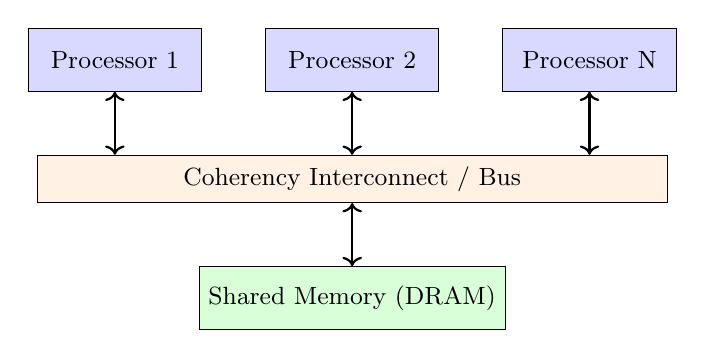
\begin{tikzpicture}[node distance=0.8cm, every node/.style={font=\small}]
        \node[draw, rectangle, fill=blue!15, minimum width=2.2cm, minimum height=0.8cm] (p1) {Processor 1};
        \node[draw, rectangle, fill=blue!15, minimum width=2.2cm, minimum height=0.8cm, right=of p1] (p2) {Processor 2};
        \node[draw, rectangle, fill=blue!15, minimum width=2.2cm, minimum height=0.8cm, right=of p2] (pn) {Processor N};

        \node[draw, rectangle, fill=orange!10, minimum width=8cm, minimum height=0.6cm, below=of p2] (bus) {Coherency Interconnect / Bus};
        
        \node[draw, rectangle, fill=green!15, minimum width=3.5cm, minimum height=0.8cm, below=of bus] (mem) {Shared Memory (DRAM)};

        \draw[<->, thick] (p1) -- (p1 |- bus.north);
        \draw[<->, thick] (p2) -- (p2 |- bus.north);
        \draw[<->, thick] (pn) -- (pn |- bus.north);
        \draw[<->, thick] (bus) -- (mem);
    \end{tikzpicture}
    \caption{Symmetric multiprocessor architecture with shared memory and coherency interconnect.}
\end{figure}

\subsubsection*{2. Communication Mechanism}
Communication is implicit. Processors read and write to the same shared address space.
If Processor 1 writes a new value to a shared variable $X$ at memory location $0x1000$, the cache coherence protocol (e.g., MESI) changes the state of Processor 1's cache line to Modified (M) and sends an invalidate signal over the bus.
When Processor 2 reads $X$, the coherence protocol intercepts the read, forces Processor 1 to write the modified data back, updates Processor 2's cache line to Shared (S), and serves the updated data, enabling communication.

\subsubsection*{3. Synchronization Mechanism}
To prevent race conditions, hardware provides atomic synchronization primitives:
\begin{itemize}
    \item \textbf{Atomic Instructions:} Operations like Compare-And-Swap (CAS) or Load-Link/Store-Conditional (LL/SC) execute read-modify-write sequences atomically.
    \item \textbf{Mutual Exclusion (Locks):} Processors acquire a lock (e.g., a spinlock) on a memory address. If the lock is held, the processor spins locally in its cache (reading the variable in Shared state). When the owner releases the lock (writing 0), the cache line is invalidated, prompting waiting processors to try to acquire the lock using atomic instructions.
\end{itemize}

\subsection*{Question 6: Compare vector processors and scalar processors in terms of architecture, execution model, and computational efficiency.}

Vector and scalar processors differ fundamentally in how they handle data arrays:

\begin{table}[htbp]
    \centering
    \begin{tabular}{lp{5.2cm}p{5.2cm}}
        \toprule
        Metric / Dimension & Scalar Processor & Vector Processor \\
        \midrule
        \textbf{Architectural Focus} & Optimized for instruction-level parallelism (ILP). Features deep pipelines, branch predictors, and out-of-order execution logic. & Optimized for data-level parallelism (DLP). Features large vector register files (e.g., 64-256 elements per register) and pipelined vector ALUs. \\
        \midrule
        \textbf{Execution Model} & \textbf{SISD/MIMD:} Fetches, decodes, and executes one instruction per scalar data element. Requires loop control code (increment, check, branch). & \textbf{SIMD-like:} A single vector instruction operates on an entire vector register (e.g., \texttt{VADD V1, V2, V3} performs 64 additions). Loop control overhead is eliminated. \\
        \midrule
        \textbf{Hazard Susceptibility} & Highly vulnerable to data hazards (requires forwarding) and control hazards (requires branch prediction). & Data hazards are resolved once for the entire vector; elements are streamed sequentially through the pipelined ALU without stalls. \\
        \midrule
        \textbf{Memory Interface} & Relies on deep cache hierarchies (L1, L2, L3) to hide memory latency. & Requires high-bandwidth memory pipelines, using techniques like memory interleaving, strided accesses, and gather-scatter operations. \\
        \midrule
        \textbf{Computational Efficiency} & Highly efficient for irregular, branching, and general-purpose applications. Poor efficiency on massive numerical datasets. & Extremely efficient for regular, scientific computations (matrix arithmetic, signal processing). Inefficient for control-flow heavy code. \\
        \bottomrule
    \end{tabular}
    \caption{Architectural comparison between scalar and vector processors.}
\end{table}

\subsection*{Question 7: Demonstrate the execution of a vector addition operation on a multivector multiprocessor.}

\subsubsection*{1. The Vector Addition Operation}
Let us compute the vector sum:
\[ \vec{C} = \vec{A} + \vec{B} \]
where the vectors contain $N = 256$ floating-point elements, and the hardware vector register length is $VL = 64$ elements.

\subsubsection*{2. Vector Loop Stripmining}
Since the vector size ($N = 256$) exceeds the hardware register length ($VL = 64$), the compiler partitions the operation into 4 chunks (stripmining):
\[ \text{Number of loops} = \frac{N}{VL} = \frac{256}{64} = 4\text{ iterations} \]

Each iteration additions a subset of indices:
\begin{itemize}
    \item Iteration 1: $i = 0 \dots 63$
    \item Iteration 2: $i = 64 \dots 127$
    \item Iteration 3: $i = 128 \dots 191$
    \item Iteration 4: $i = 192 \dots 255$
\end{itemize}

\subsubsection*{3. Execution on a Multiprocessor}
In a \textbf{multivector multiprocessor}, these 4 loop iterations are distributed across different vector processors to execute in parallel:

\begin{figure}[htbp]
    \centering
    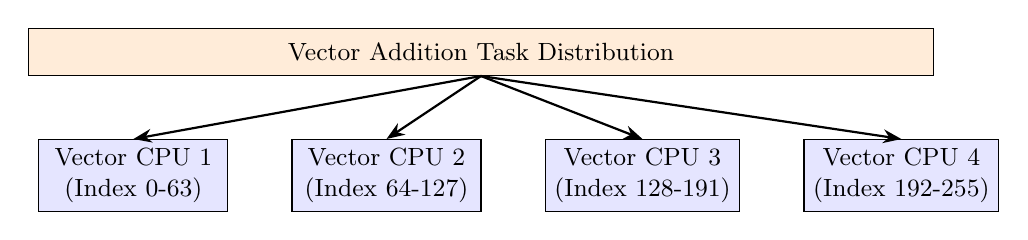
\begin{tikzpicture}[node distance=0.8cm, every node/.style={font=\small}]
        \node[draw, rectangle, fill=blue!10, minimum width=2.4cm, minimum height=0.8cm, align=center] (v1) {Vector CPU 1\\(Index 0-63)};
        \node[draw, rectangle, fill=blue!10, minimum width=2.4cm, minimum height=0.8cm, align=center, right=of v1] (v2) {Vector CPU 2\\(Index 64-127)};
        \node[draw, rectangle, fill=blue!10, minimum width=2.4cm, minimum height=0.8cm, align=center, right=of v2] (v3) {Vector CPU 3\\(Index 128-191)};
        \node[draw, rectangle, fill=blue!10, minimum width=2.4cm, minimum height=0.8cm, align=center, right=of v3] (v4) {Vector CPU 4\\(Index 192-255)};

        \node[draw, rectangle, fill=orange!15, minimum width=11.5cm, minimum height=0.6cm, above=of v2.north, xshift=1.2cm] (dist) {Vector Addition Task Distribution};

        \draw[-{Stealth}, thick] (dist.south) -- (v1.north);
        \draw[-{Stealth}, thick] (dist.south) -- (v2.north);
        \draw[-{Stealth}, thick] (dist.south) -- (v3.north);
        \draw[-{Stealth}, thick] (dist.south) -- (v4.north);
    \end{tikzpicture}
    \caption{Parallel vector task distribution on a multivector multiprocessor.}
\end{figure}

\subsubsection*{4. Pipeline Execution Model within each Vector CPU}
Within a single Vector CPU (e.g., Vector CPU 1 processing indices $0 \dots 63$):
\begin{enumerate}
    \item \textbf{Vector Load:} Loads $V_A \leftarrow A[0 \dots 63]$ and $V_B \leftarrow B[0 \dots 63]$.
    \item \textbf{Pipelined Execution:} The operation \texttt{VADD V\_C, V\_A, V\_B} is fetched. The elements stream through the vector adder pipeline:
    \begin{itemize}
        \item \textbf{Cycle 1:} Element $0$ enters stage 1 (exponent compare).
        \item \textbf{Cycle 2:} Element $1$ enters stage 1; Element $0$ moves to stage 2 (mantissa add).
        \item \textbf{Cycle 5 (steady state):} The pipeline is full (assuming 4 stages). Result element $C[0]$ is output, and subsequent results are output at a rate of \textbf{1 result element per cycle}.
    \end{itemize}
    \item \textbf{Vector Store:} The vector register $V_C$ is written back to main memory $C[0 \dots 63]$.
\end{enumerate}

By distributing the stripminded loops across the 4 vector processors, the entire addition is completed in parallel, achieving both spatial parallelism (across multiple processors) and temporal parallelism (via arithmetic pipelining).

\end{document}
